\clearpage
\begin{figure}[h]
  \centering
    \subfigure[]{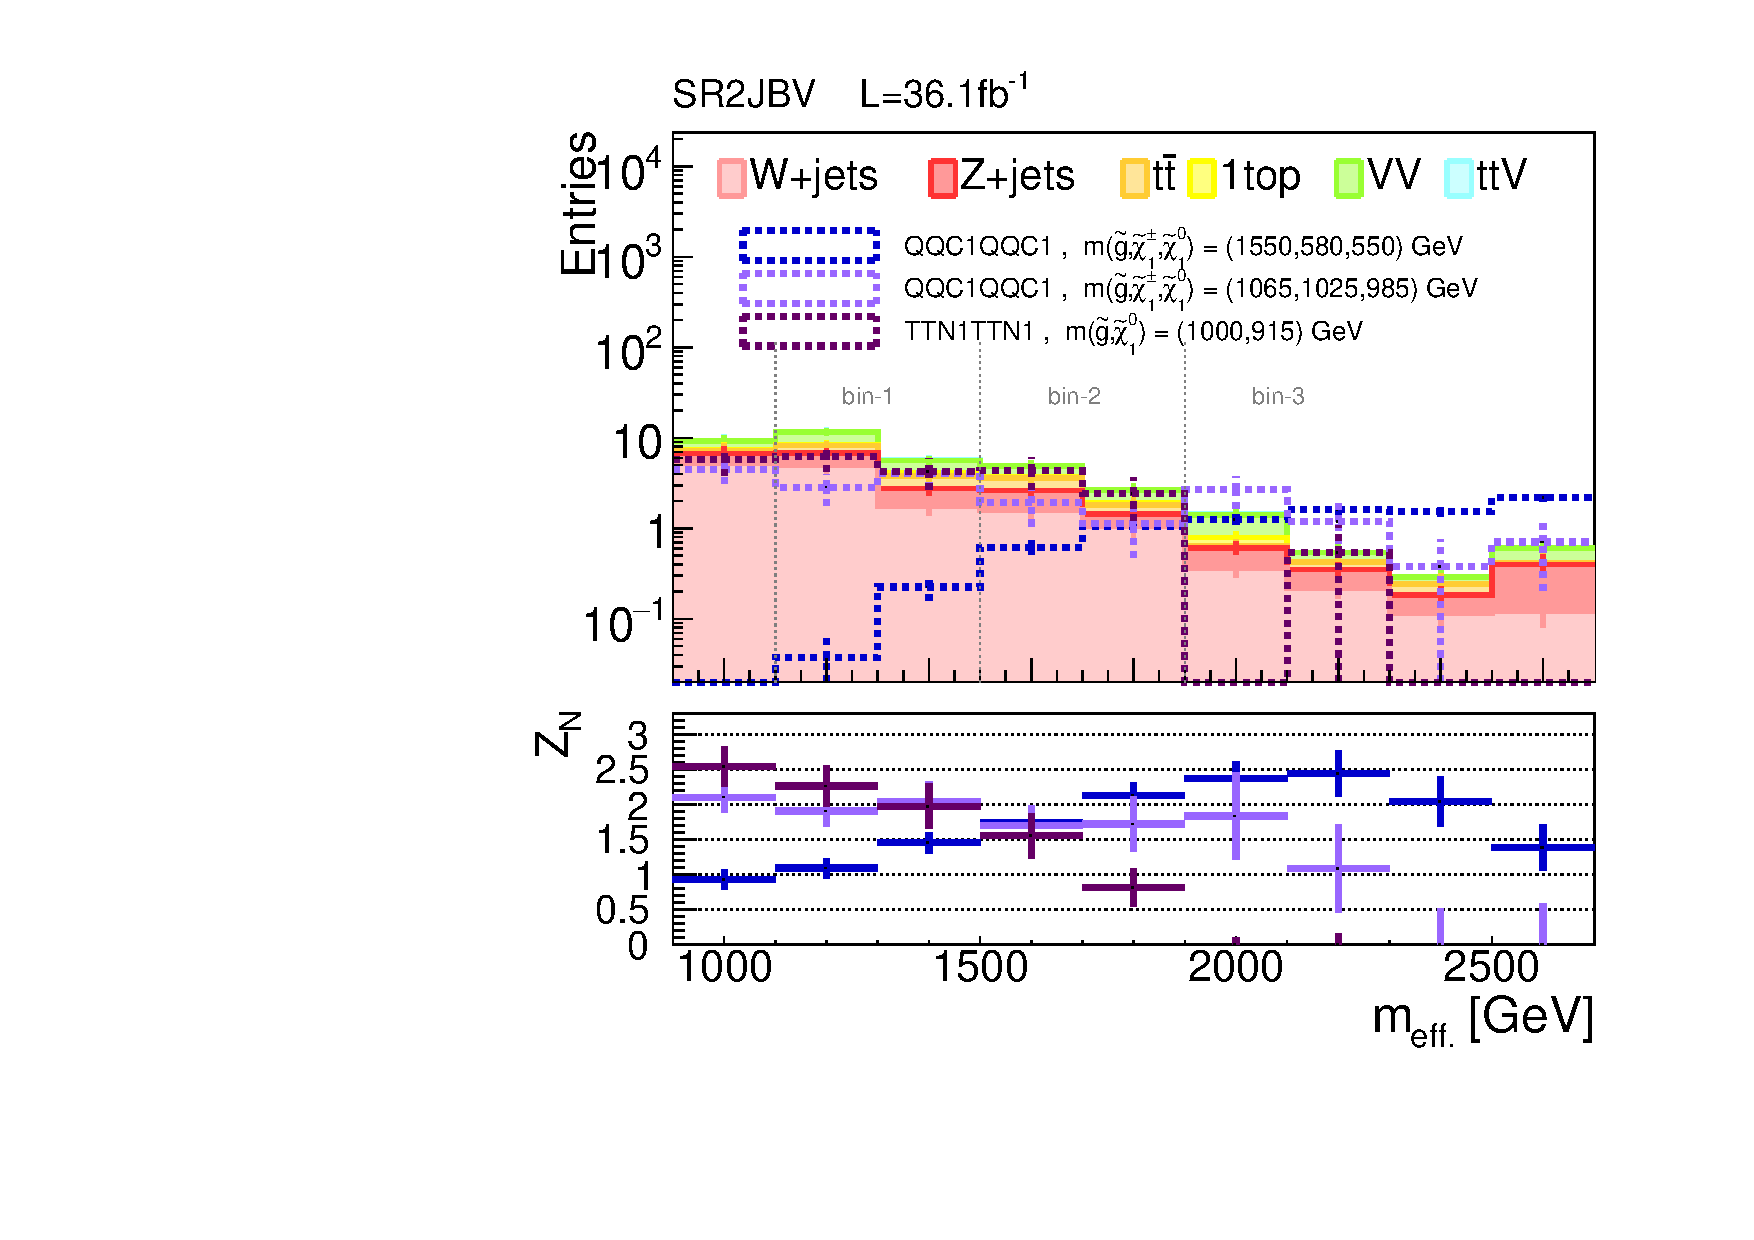
\includegraphics[width=0.45\textwidth]{figures/SRdefinition/N1plot/meffInc30_2JMEFFInclBV.pdf}}
    \subfigure[]{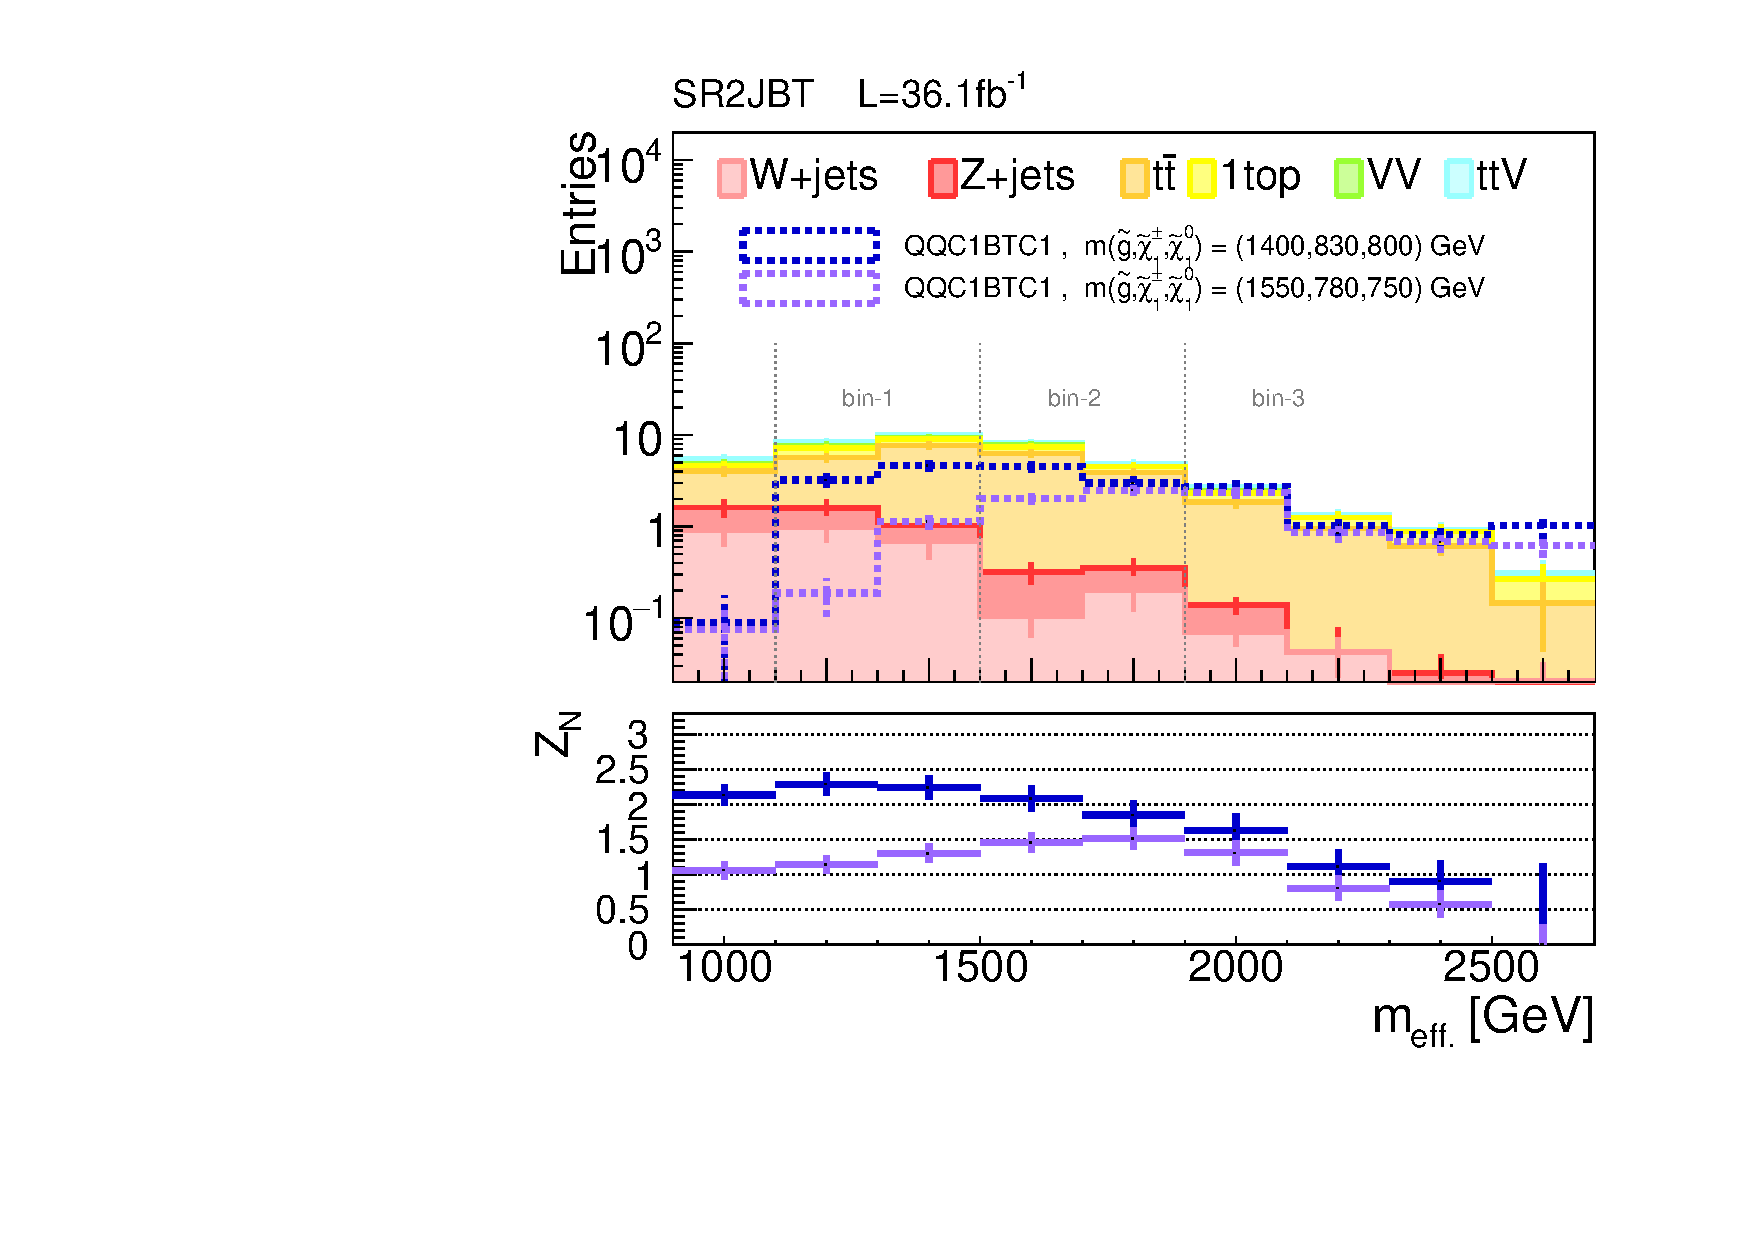
\includegraphics[width=0.45\textwidth]{figures/SRdefinition/N1plot/meffInc30_2JMEFFInclBT.pdf}}
    \caption{
     $\meffInc$ distribution in the (a) b-vetoed (BV) and (b) b-tagged (BT) slices of the optimized \textbf{2J} signal region. Bottom row display the sensitivity $Z_N := S/\sqrt{B+\alpha^2 B^2}$ for each reference signals.
    \label{fig::SRdefinition::SRmeffInc2J}}
\end{figure}

\begin{figure}[h]
  \centering
    \subfigure[]{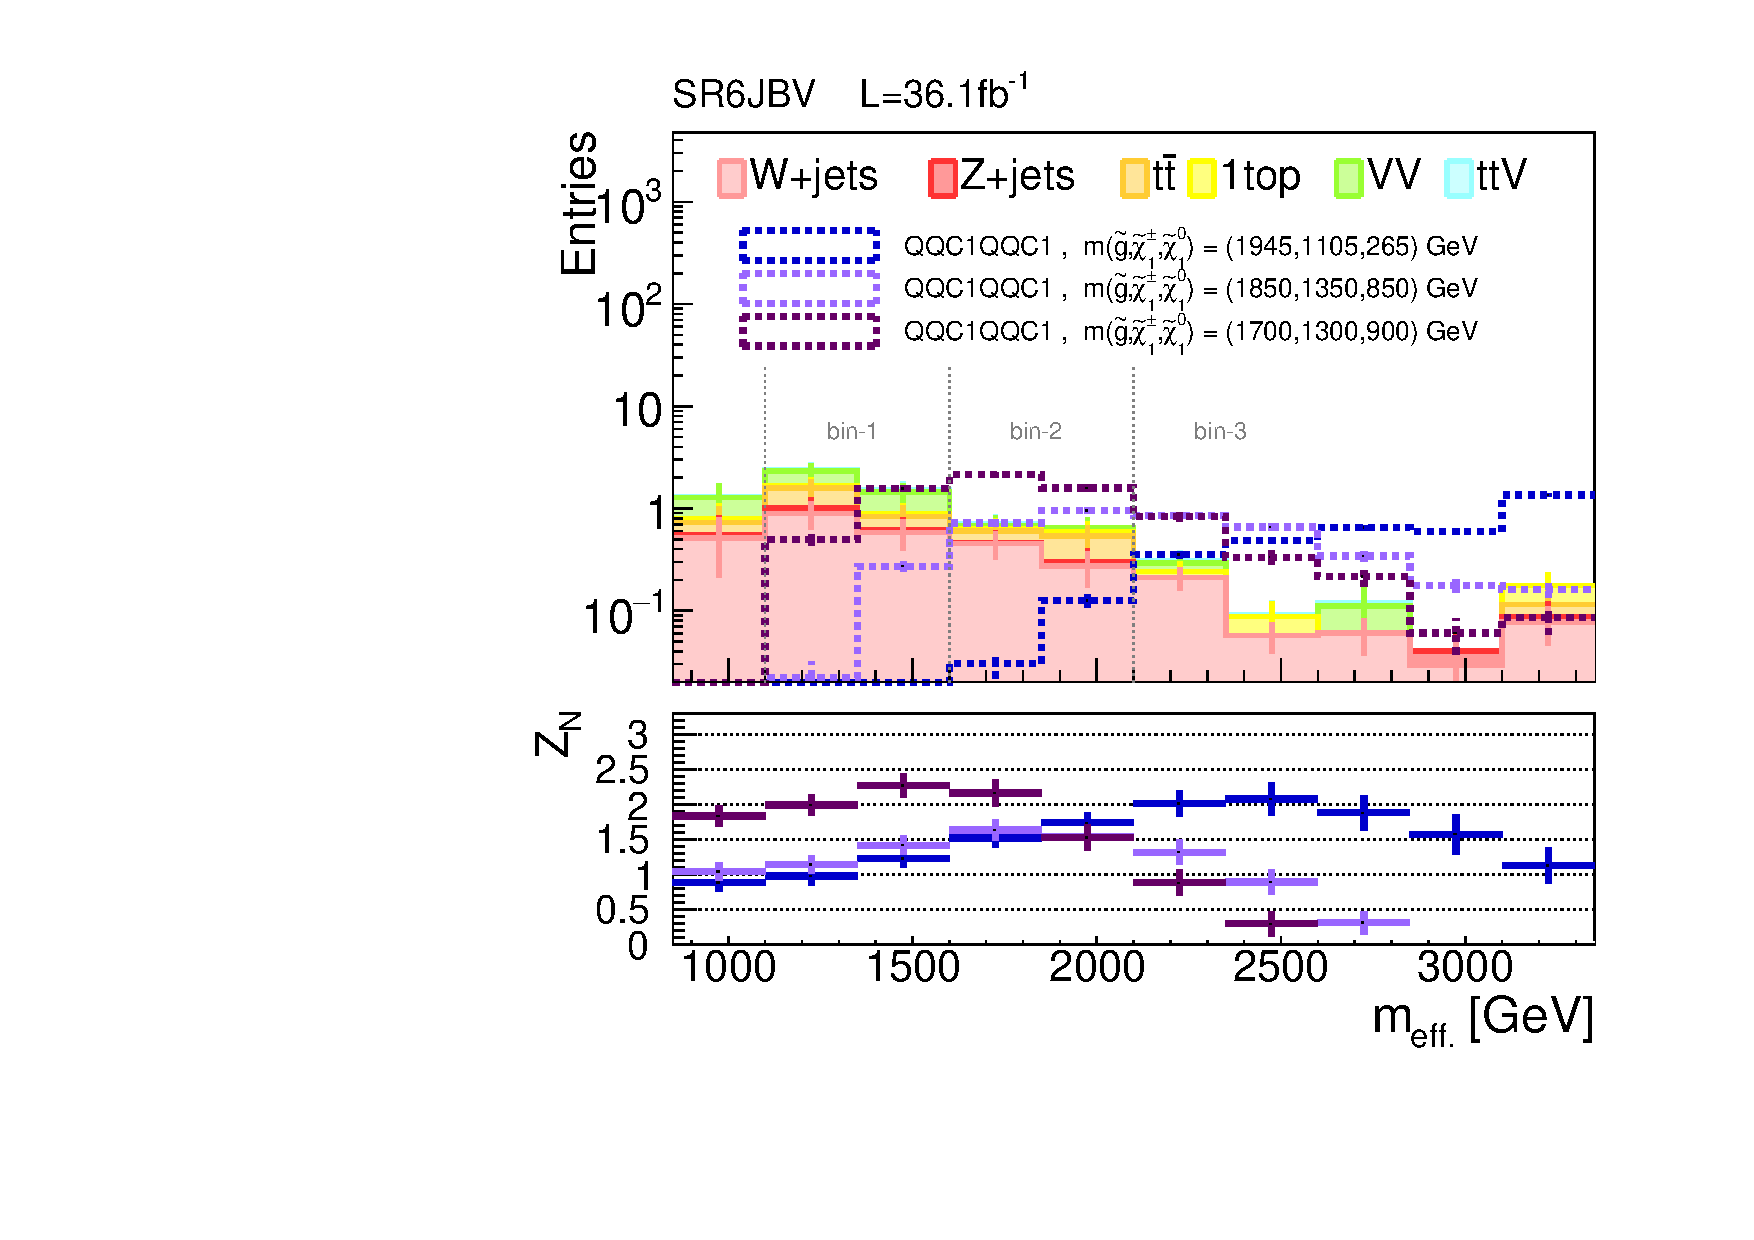
\includegraphics[width=0.45\textwidth]{figures/SRdefinition/N1plot/meffInc30_6JMEFFInclBV.pdf}}
    \subfigure[]{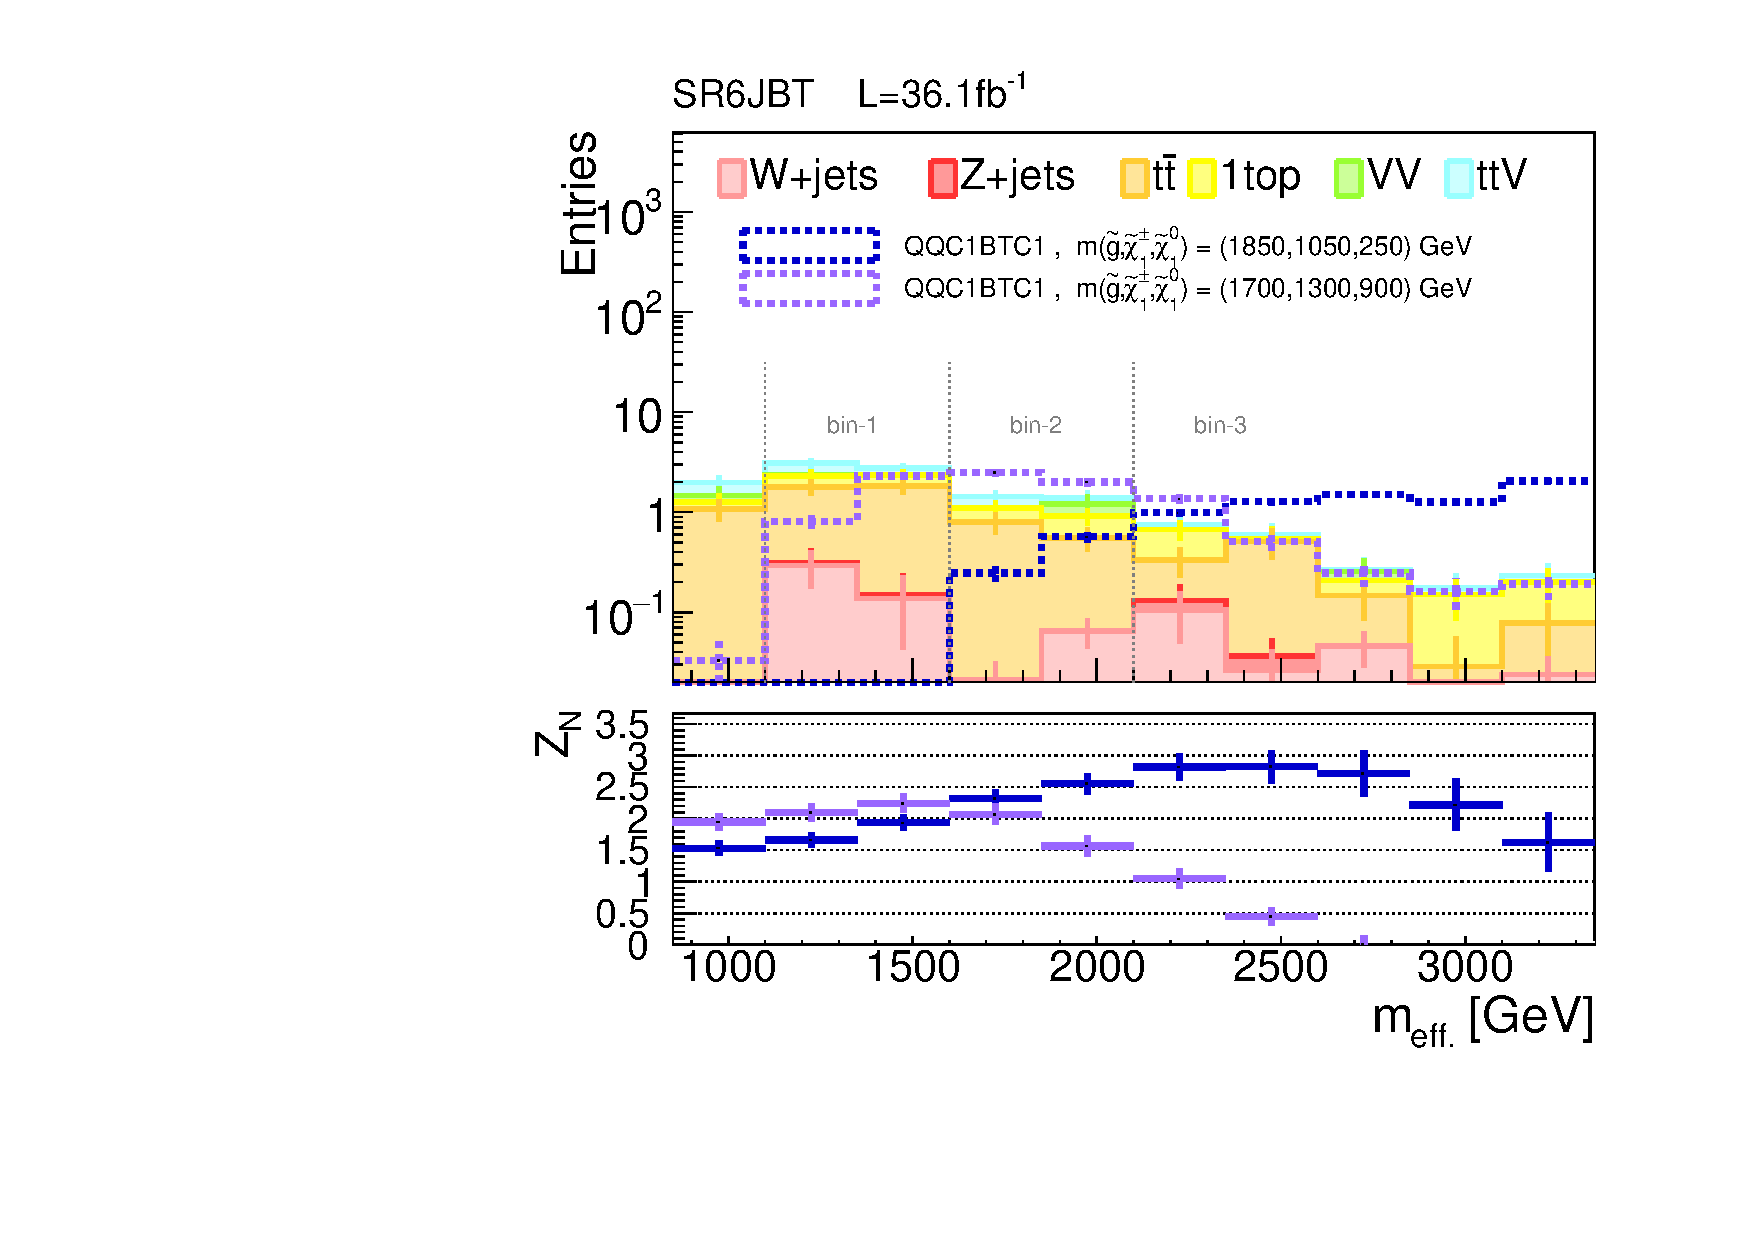
\includegraphics[width=0.45\textwidth]{figures/SRdefinition/N1plot/meffInc30_6JMEFFInclBT.pdf}}
    \caption{ 
     $\meffInc$ distribution in the (a) b-vetoed (BV) and (b) b-tagged (BT) slices of the optimized \textbf{6J} signal region. Bottom row display the sensitivity $Z_N := S/\sqrt{B+\alpha^2 B^2}$ for each reference signals.
    \label{fig::SRdefinition::SRmeffInc6J} }
\end{figure}

\clearpage
\begin{figure}[h]
  \centering
    \subfigure[]{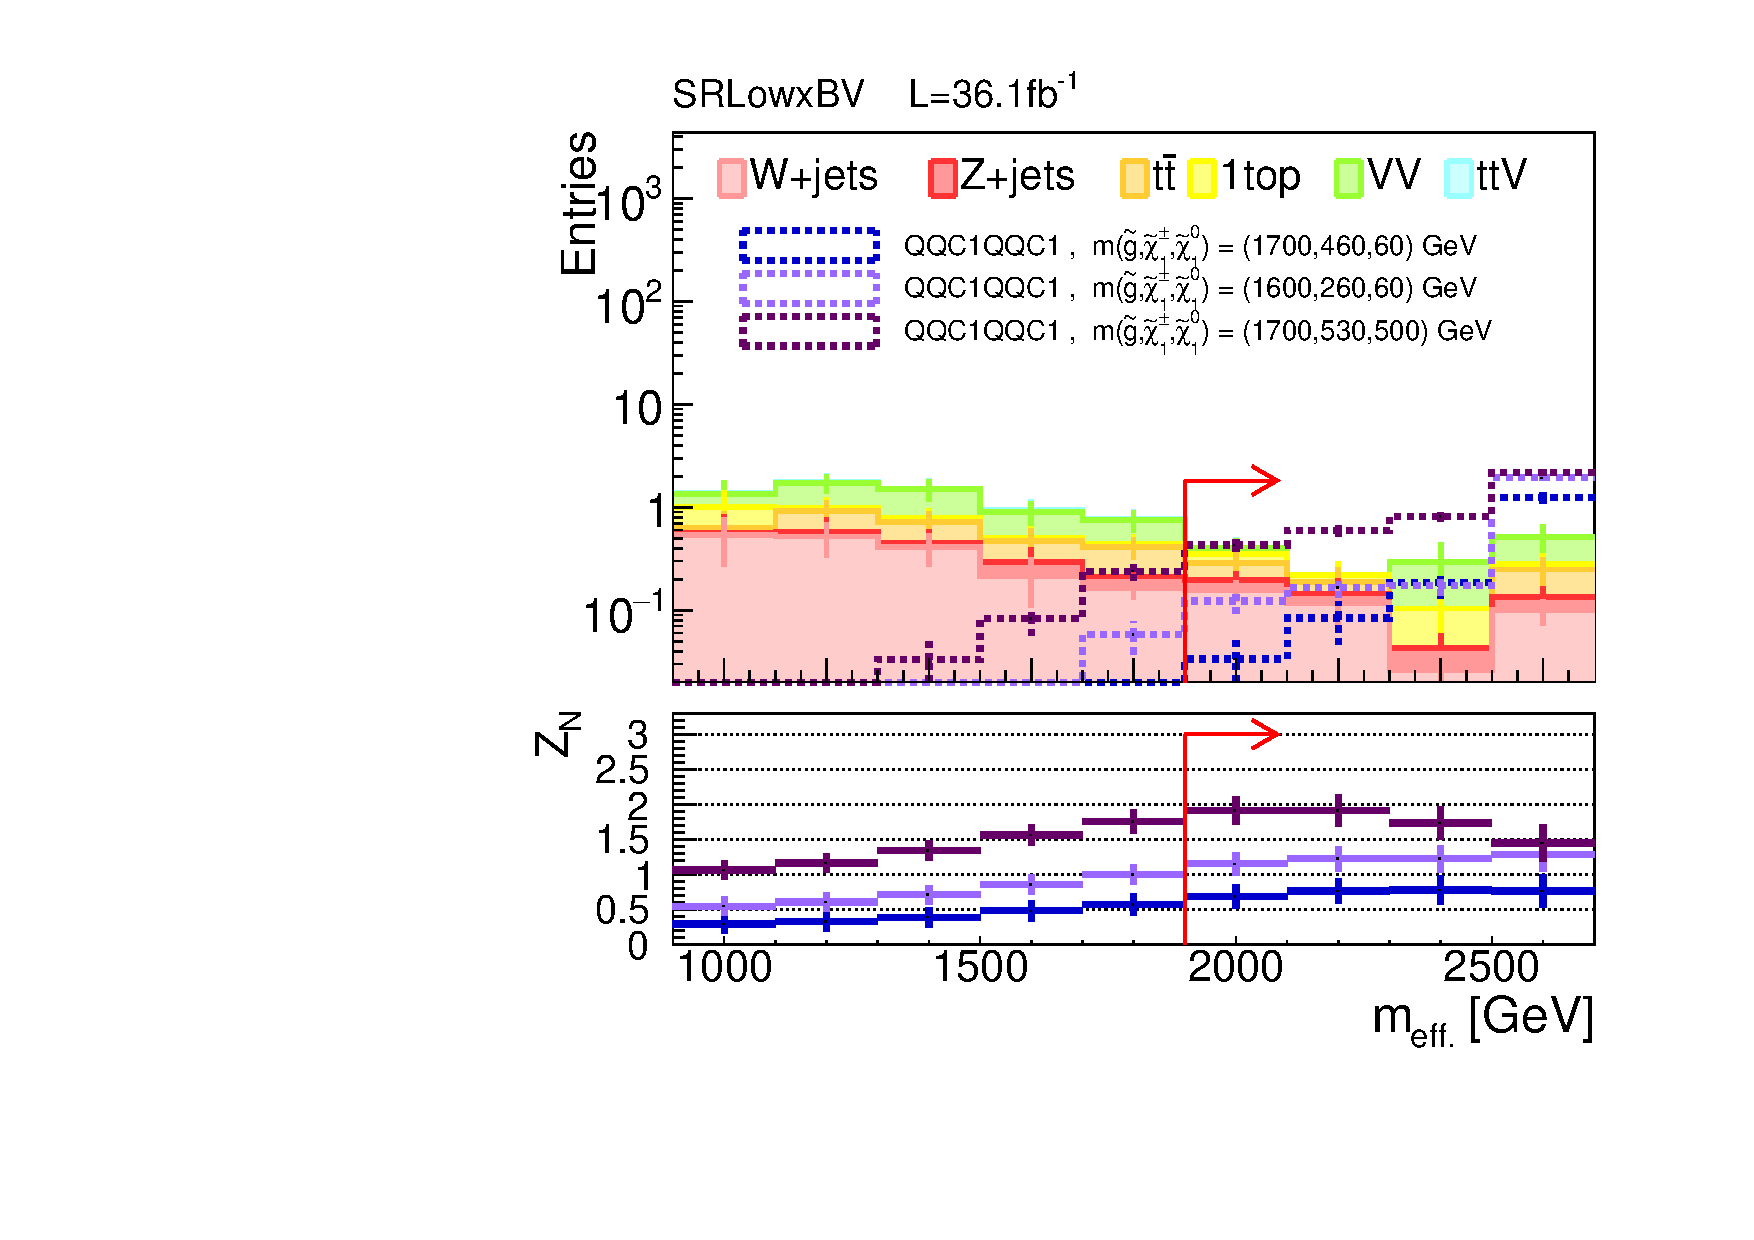
\includegraphics[width=0.41\textwidth]{figures/SRdefinition/N1plot/meffInc30_LowxBV.pdf}}
    \subfigure[]{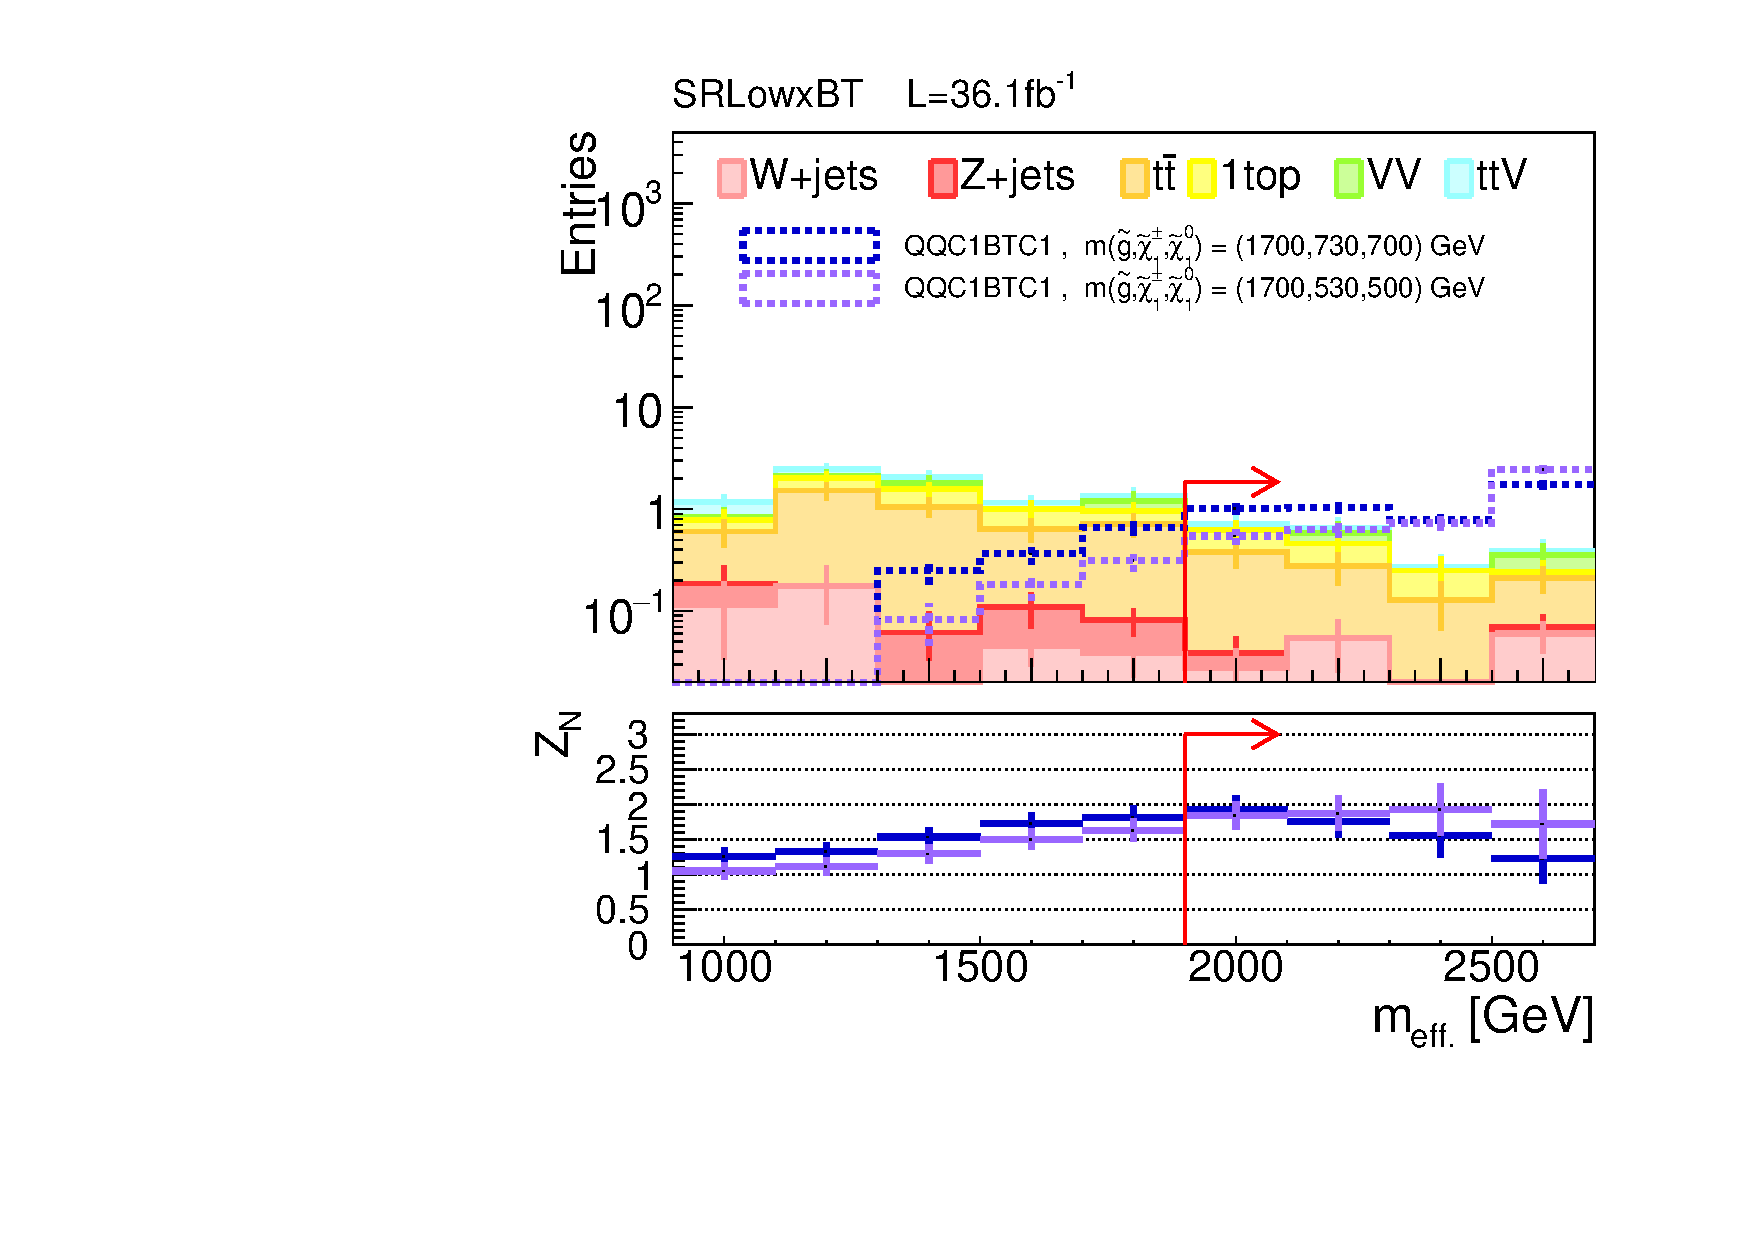
\includegraphics[width=0.41\textwidth]{figures/SRdefinition/N1plot/meffInc30_LowxBT.pdf}}
    \caption{ 
     $\meffInc$ distribution in the (a) b-vetoed (BV) and (b) b-tagged (BT) slices of the optimized \textbf{Low-x} signal region. The red arrow indicates the cut position of $\meffInc$. Bottom row display the sensitivity $Z_N := S/\sqrt{B+\alpha^2 B^2}$ for each reference signals.
    \label{fig::SRdefinition::SRmeffIncLowx}}
\end{figure}

\begin{figure}[h]
  \centering
    \subfigure[]{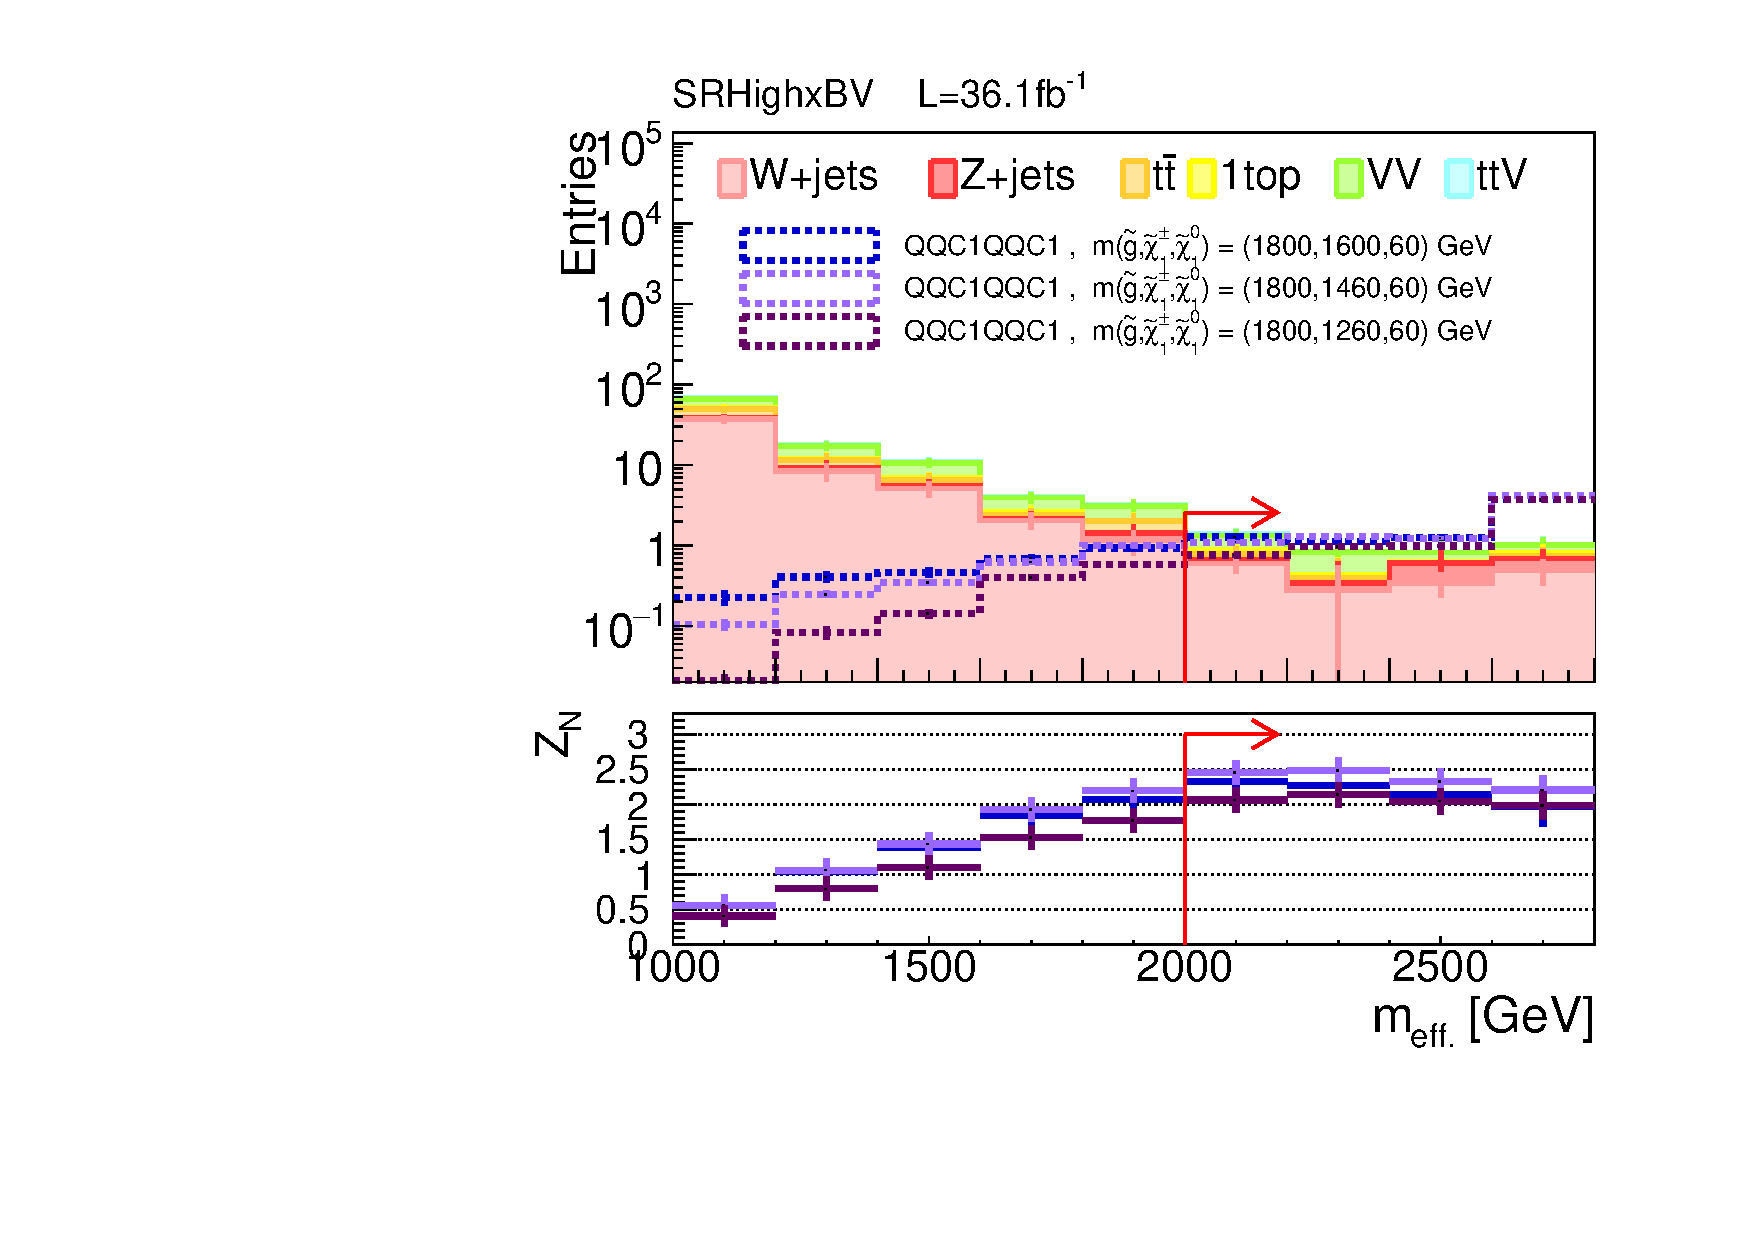
\includegraphics[width=0.41\textwidth]{figures/SRdefinition/N1plot/meffInc30_HighxBV.pdf}}
    \subfigure[]{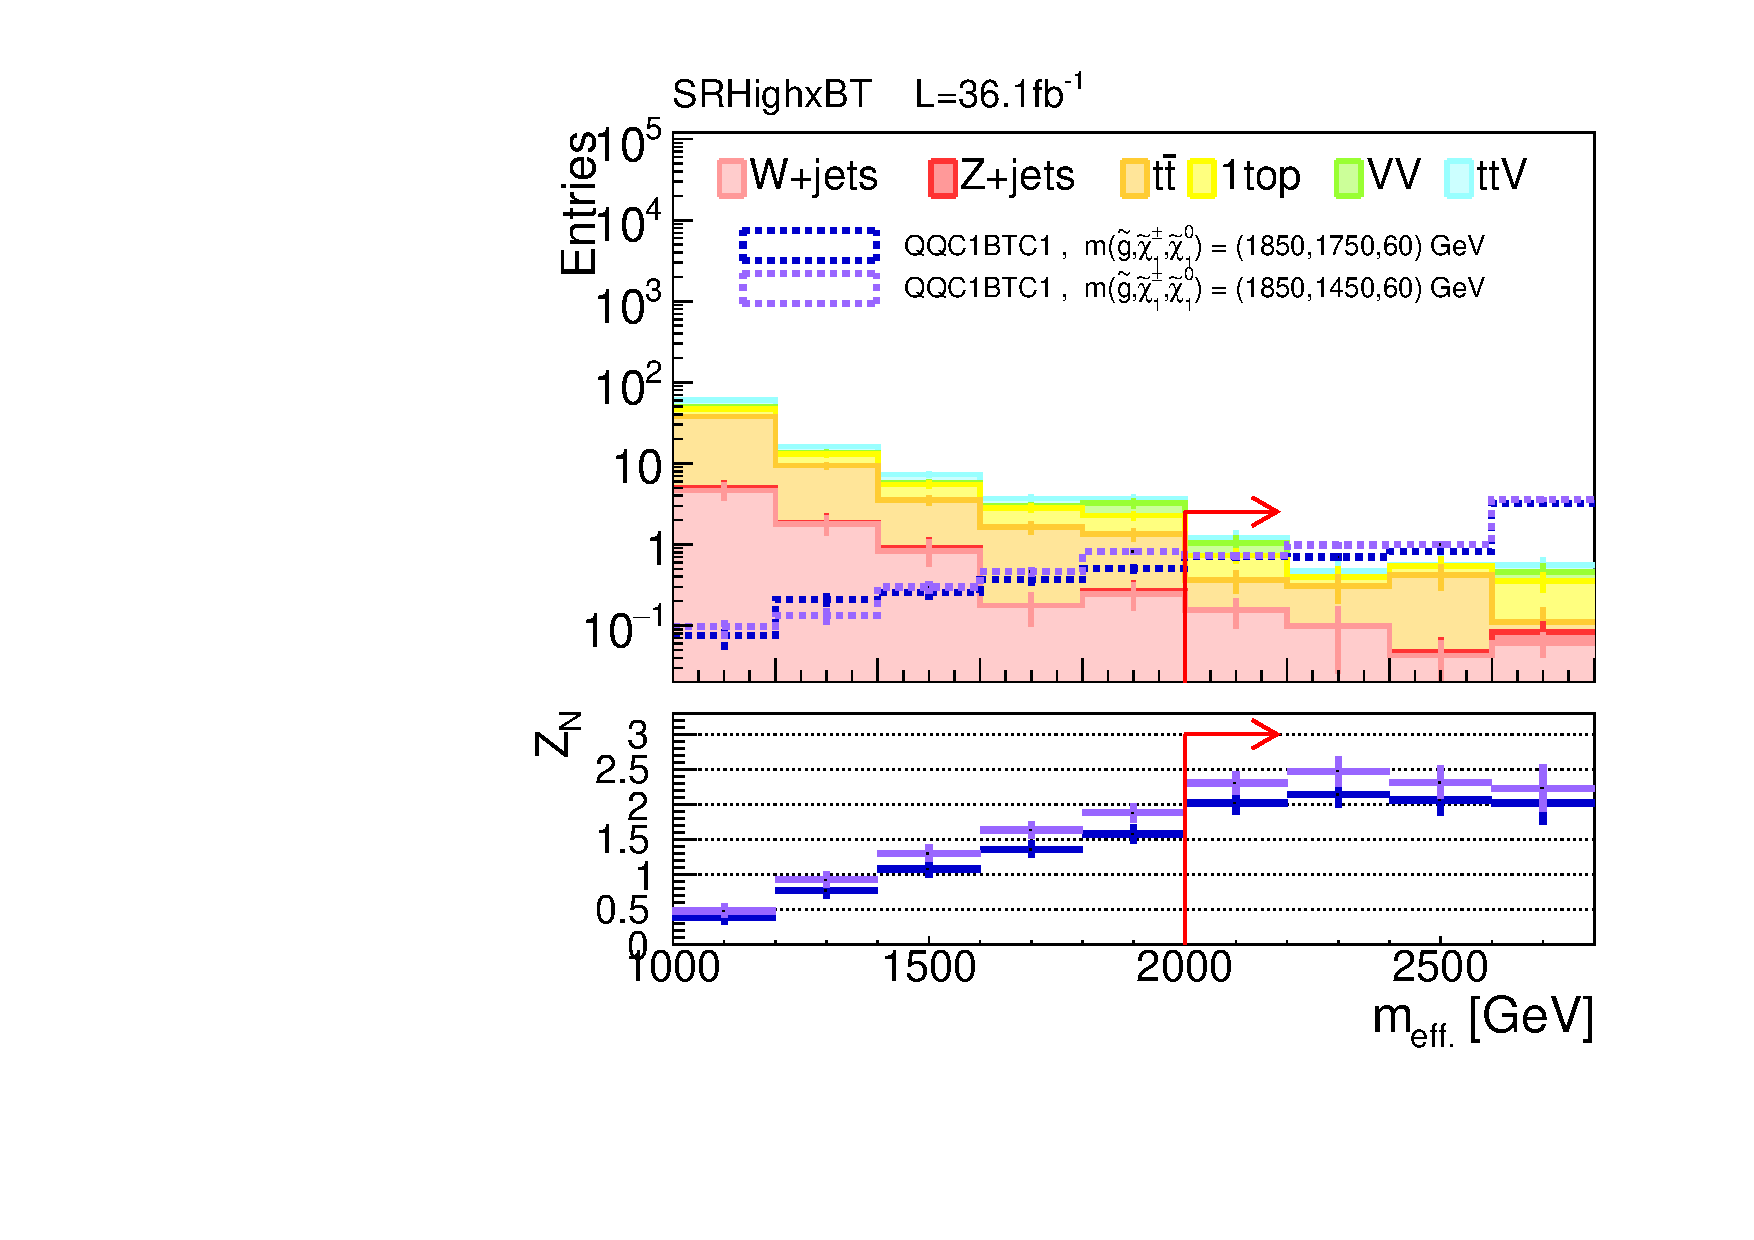
\includegraphics[width=0.41\textwidth]{figures/SRdefinition/N1plot/meffInc30_HighxBT.pdf}}
    \caption{ 
     $\meffInc$ distribution in the (a) b-vetoed (BV) and (b) b-tagged (BT) slices of the optimized \textbf{High-x} signal region. The red arrow indicates the cut position of $\meffInc$. Bottom row display the sensitivity $Z_N := S/\sqrt{B+\alpha^2 B^2}$ for each reference signals.
    \label{fig::SRdefinition::SRmeffIncHighx}       }
\end{figure}

\clearpage
\begin{figure}[h]
  \centering
    \subfigure[]{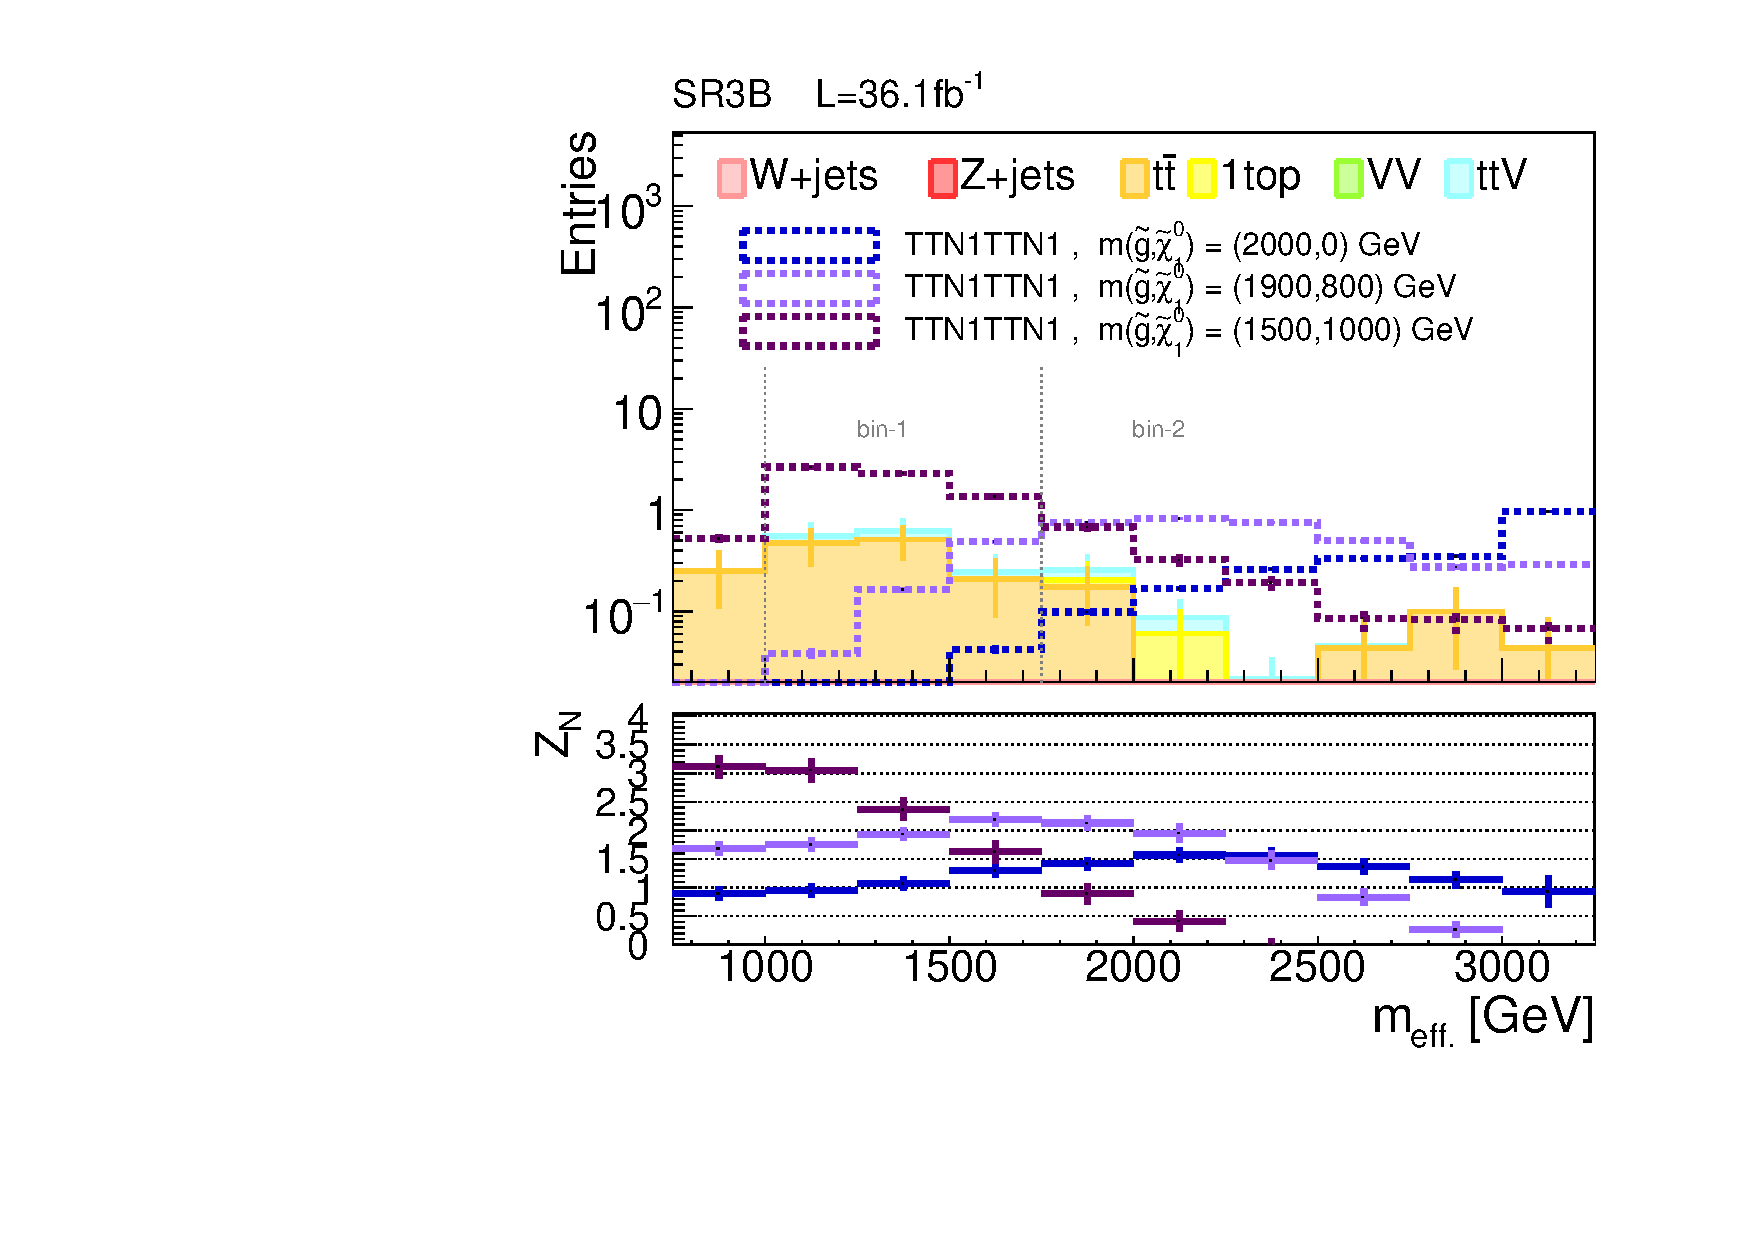
\includegraphics[width=0.95\textwidth]{figures/SRdefinition/N1plot/meffInc30_3BMEFFIncl.pdf}}
    \caption{ 
     $\meffInc$ distribution in the (a) b-vetoed (BV) and (b) b-tagged (BT) slices of the optimized \textbf{3B} signal region. Bottom row display the sensitivity $Z_N := S/\sqrt{B+\alpha^2 B^2}$ for each reference signals.
    \label{fig::SRdefinition::SRmeffInc3B}}
\end{figure}
